\documentclass[10pt]{article}
\usepackage[utf8]{inputenc}
\usepackage[swedish,english]{babel}
\usepackage[margin=2cm]{geometry}
\usepackage[utf8]{inputenc}
\usepackage{graphicx}
\graphicspath{ {images/} }
\selectlanguage{swedish}

\title{Kravspecifikation}

\author{
    Joel Almqvist\\
    \texttt{joeal360@student.liu.se}
    \and
    Björn Detterfelt\\
    \texttt{bjode786@student.liu.se}
    \and
    Tim Håkansson\\
    \texttt{timha404@student.liu.se}
    \and
    David Kjellström\\
    \texttt{davkj168@student.liu.se}
    \and
    Axel Löjdquist\\
    \texttt{axelo225@student.liu.se}
    \and
    Joel Oskarsson\\
    \texttt{joeos014@student.liu.se}
    \and
    Lieth Wahid\\
    \texttt{liewa893@student.liu.se}
    \and
    Alexander Wilkens\\
    \texttt{alewi684@student.liu.se}
}

\begin{document}

\maketitle
\pagebreak
\tableofcontents
\pagebreak
\section{Inledning}
	I detta kapitel definieras och introduceras kontexten för projektet som ska utföras.

	\subsection{Definitioner}
		\begin{itemize}
		\item User Interface (UI) -- Den del av applikationen som visar spelplanen
		\item Kontroller -- En mobil eller surfplatta som kör kontrolldelen av applikationen
		\item HotJoin -- möjligheten att hoppa in i ett pågående spel
		\item Standard nätverks förhållande - Stabilt WiFi-LAN kopplad till en router med stabil ethernet uppkoppling.
		\item Sensor -- En sensor som sitter på kontrollern som inte är en touch-skärm (t.ex. en accelerometer)
		\item Vanliga nätverksförhållanden -- Stabil nätverksuppkoppling utan yttre störningar.
		\end{itemize}	

	\subsection{Parter}
	Kunden till projektet är Cybercom Sweden. Projektet utförs av projektgruppens medlemmar.
	\subsection{Syfte \& mål}
		Syftet med projektet är att skapa en prototyp för att demonstrera Cybercoms IoT backend. För att kunna uppnå detta, ska ett realtids multiplayerspel skapas. Projektgruppens syfte är att genomföra ett kandidatarbete kan utföras enligt kursen TDDD96 -- Kandidatprojekt i programvaruutveckling mål.
	
	\subsection{Användning}
		Mobil eller surfplatta ska användas som kontroll för spelet medan UI:t ska användas på en enhet med stor skärm för att visa spelplanen.
	
	\subsection{Bakgrundsinformation}
		Projektgruppen har tidigare läst en kurs om programutvecklingsmetodik och vill omsätta denna kunskap i praktiken. 
		
\pagebreak
\section{Översikt av Systemet}
	Detta kapitel ger en överskådlig blick av systemet.

	\subsection{Grov beskrivning av produkten}
	Produkten ska vara ett realtids multiplayerspel. Spelet är uppdelat i två olika komponenter, en UI del och en kontroller del. UI delen är tänkt att agera som skärm för spelet,  Dessa två komponenter ska enbart kommunicera med varandra genom Cybercoms backend, se figur 1. En kontroller kan t.ex. vara en mobilenhet och ska styras av dess sensorer. Både kontroller och UI:t ska vara progressiva webbappar. 
	
	\begin{figure}[h]
		\centering
		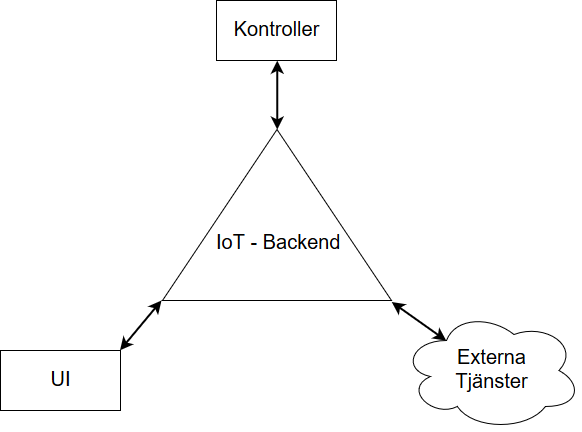
\includegraphics[scale=0.4]{backend}
		\caption{kommunikation mellan Cybercoms backend och komponenterna i systemet}
		\label{fig:backend}
	\end{figure}
	
	
	\subsection{Beroenden av andra system}
	Produkten är beroende av Cybercoms backend då all kommunikation måste gå genom denna. Produkten är även beroende av en enhet som har tillgång till senaste versionen av Chrome samt en enhet som kan köra UI delen av systemet.

\pagebreak
\section{Funktionella Krav}
	Detta avsnitt listar de funktionella kraven på produkten.	
	
	\begin{tabular}{| p{2cm} | p{8cm} | p{2cm}|}
		\hline
		
		\textbf{Krav nr.} & \textbf{Beskrivning} &\textbf{Prioritet} \\ \hline
		Krav 1 & Telefon/Platta ska användas som kontroller för spelet. & 1 \\ \hline
		Krav 2 & Applikationen ska stödja ett minimum av 2 antal användare & 1 \\ \hline
		Krav 3 & Applikationen ska köras i realtid & 1 \\ \hline
		Krav 4 & Applikationen ska kunna köras på en enhet som har chrome & 1 \\ \hline
		Krav 5 & UI ska endast kommunicera med Cybercoms backend & 1 \\ \hline
		Krav 6 & Applikationen ska stödja version 64 av Chrome & 1 \\ \hline
		Krav 7 & En användare ska kunna gå in i en spelinstans & 1 \\ \hline
		Krav 8 & Applikationen ska stödja Hotjoinfunktionalitet & 1 \\ \hline
		Krav 9 & Flera instanser av spelet ska kunna köras samtidigt & 1 \\ \hline
		Krav 10 & Applikationen ska stödja styrning med tagentbord och mus & 2 \\ \hline
		
		
	\end{tabular}
	
\section{Designkrav}
	Detta avsnitt listar kraven på utvecklingsprocessen
	
	\begin{tabular}{| p{2cm} | p{8cm} | p{2cm}|}
		\hline
		\textbf{Krav nr.} & \textbf{Beskrivning} & \textbf{Prioritet} \\ \hline
		Krav 11 & All kod ska följa två mellanslags indentering & 1\\ \hline
		Krav 12 & All kod som körs i webbläsaren ska vara Javascript & 1 \\ \hline
		Krav 13 & Applikationen ska utvecklas som en PWA & 1 \\ \hline
		Krav 14 & Koden ska följa en dokumentationsstandard & 1 \\ \hline
		Krav 15 & UI och Kontrollerns kod ska licensieras under MITs opensource licens & 1 \\ \hline
		Krav 16 & Applikationen sa föla Javascript ES2015+ & 1 \\ \hline
	\end{tabular}

\section{Kvalitetskrav}
	Detta avsnitt listar krav på kvalitén hos den slutgilitga produkten.
	
		\begin{tabular}{|p{2cm}|p{8cm}|p{2cm}|}
		\hline
		\textbf{Krav nr.} & \textbf{Beskrivning} & \textbf{Prioritet} \\ \hline
		Krav 17 & Tiden från att en användare utför en handling från kontrollern till den visuella responsen från UI:t får inte överskrida 1 sekund under vanliga nätverksförhållanden & 1\\ \hline
		Krav 18 & UI:t ska kunna köras i 4 timmar utan avbrott & 1 \\ \hline
		Krav 19 & Arkitekturen för systemet ska vara designat så att det är möjligt att vidareutveckla projektet & 1 \\ \hline
		Krav 20 & Tiden att ansluta sig till en spelsession får inte överskrida 10 sekunder under vanliga nätverksförhållanden & 1 \\ \hline
		
	\end{tabular}

\end{document}